\documentclass[12pt,a4paper]{article}

\usepackage[left=3cm, right=3cm, top=2.5cm, bottom=2.5cm]{geometry}
\usepackage{setspace}
\usepackage{amsmath}
\usepackage{tikz}
\usepackage{pgfplotstable}
\usepackage{titlesec}
\usepackage{bm}
\usepackage{tcolorbox}
\tcbuselibrary{skins}
\usepackage{empheq}
\usepackage{booktabs}
\usepackage{caption}
\usepackage{hyperref}
\usepackage{fancyhdr}
\hypersetup{
    colorlinks=true,
    linkcolor=black,
    filecolor=magenta,      
    urlcolor=cyan,
    pdfpagemode=FullScreen,
    }
\usepackage{graphicx}
\graphicspath{ {./images/} }


\titleformat{\section}{\Large\bfseries}{\thesection}{1em}{}
\titleformat{\subsection}{\large\bfseries}{\thesubsection}{1em}{}


\renewcommand{\contentsname}{Table des Matières}
\renewcommand{\tablename}{Tableau }
%\renewcommand{\baselinestretch}{1.5}

\title{#Titlu#}
\author{Liviu Arsenescu, Cătălin Bozan}
\date{date}

\newtcbox{\mymath}[1][]{%
    nobeforeafter,
    math upper,
    tcbox raise base,
    enhanced,
    colframe=black,
    colback=white,
    boxrule=1pt,
    drop shadow={
        shadow xshift=3pt,
        shadow yshift=-3pt,
        opacity=1
    },
    #1
}

\pagestyle{fancy}
\fancyhf{}
\rhead{
\includegraphics[width=4cm]{hearclogo.png}}
\lhead{\thepage}
\setlength{\headsep}{30pt}

\begin{document}
    \pagenumbering{gobble}
    \begin{titlepage}
        \begin{center}
            \vspace*{\fill}
            \Huge \textbf{#Titlu#} \\
            \Huge \textbf{#Subtitlu#} \\
            \Large Rapport du Laboratoire \\
            \begin{figure}[h]
                \centering
                
\includegraphics[width=7cm]{hearclogo.png}
            \end{figure}
            \vspace{\fill}
            \Large Liviu Arsenescu, Cătălin Bozan \\
            09.04.2024

            \vspace*{\fill}
        \end{center}
    \end{titlepage}

    \thispagestyle{empty}
    \tableofcontents
    \newpage

    \pagenumbering{arabic}
    \section{Description de l'expérience}
    \subsection{Buts}
    \begin{itemize}
        \item Étude du comportement des ondes stationnaires.
        \item Application et comparaison de méthodes de calcul de la vitesse de propagation d'une onde dans une corde élastique.
    \end{itemize}

    \subsection{Éléments théoriques}
    \subsubsection{Les différentes grandeurs physiques rencontrées}
    \begin{minipage}{0.6\linewidth}
        \begin{itemize}
            \item Différentes longueurs ($\bm{L, l', l''}$)
            \item Différentes masses ($\bm{m, m_c}$)
            \item Force de la pesanteur ($\bm{F}$)
            \item Tension dans la corde ($\bm{F_T}$)
            \item Masse linéique de la corde ($\bm{\mu}$)
            \item Fréquence de l'harmonique $n$ ($\bm{f_n}$)
            \item Période d'oscillation $n$ ($\bm{T}$)
        \end{itemize}
    \end{minipage}%
    \hfill
    \begin{minipage}{0.4\linewidth}
        \begin{itemize}
            \item[-] $\bm{[l]} =$ m
            \item[-] $\bm{[m]} =$ g
            \item[-] $\bm{[F]} =$ N
            \item[-] $\bm{[F_T]} =$ N
            \item[-] $\bm{[\mu]} =$ gm$^{-1}$
            \item[-] $\bm{[f_n]} =$ Hz
            \item[-] $\bm{[T]} =$ s
        \end{itemize}   
    \end{minipage}

    \subsubsection{Vitesse de propagation de l'onde dans la corde}
    On prends un morceau de corde et considère que $F_T$ est la tension de la corde qui est équivalente à la force gravitationnelle du poids $F$ et la masse linéique de la corde $\mu$.
    
    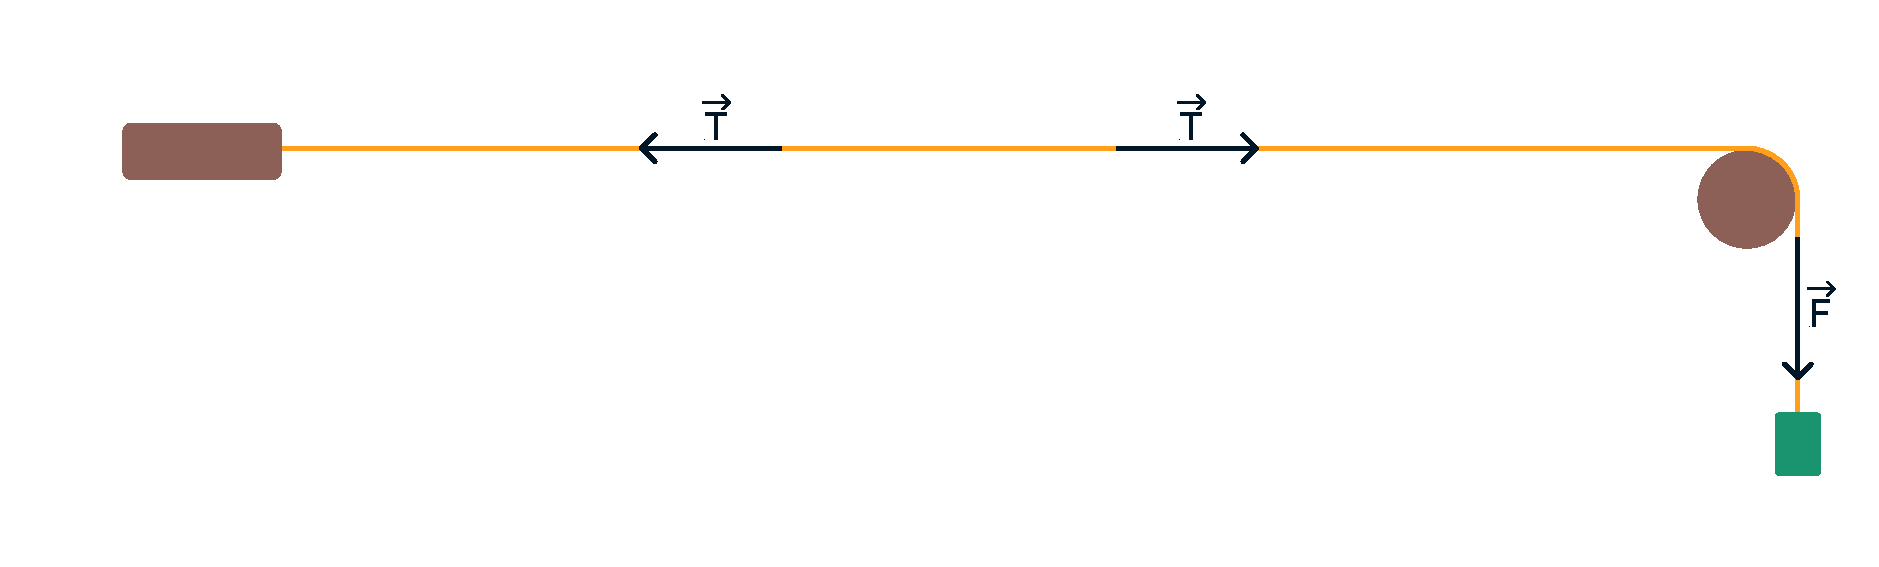
\includegraphics[width=.7\paperwidth]{images/schema_static_force.pdf}

    Si nous considérons un morceau de corde en mouvement, nous pouvons prendre deux points ($A$ et $B$) sur la corde et analyser les forces qui agissent sur eux ($F_a$ et $F_b$).

    Les deux forces $F_a$ et $F_b$ sont équivalentes à la tension dans la corde $F_T$.

    \begin{empheq}[box={\mymath}]{align*}
        \lvert F_a \rvert &= \lvert F_b \rvert = \lvert F_T \rvert
    \end{align*}

    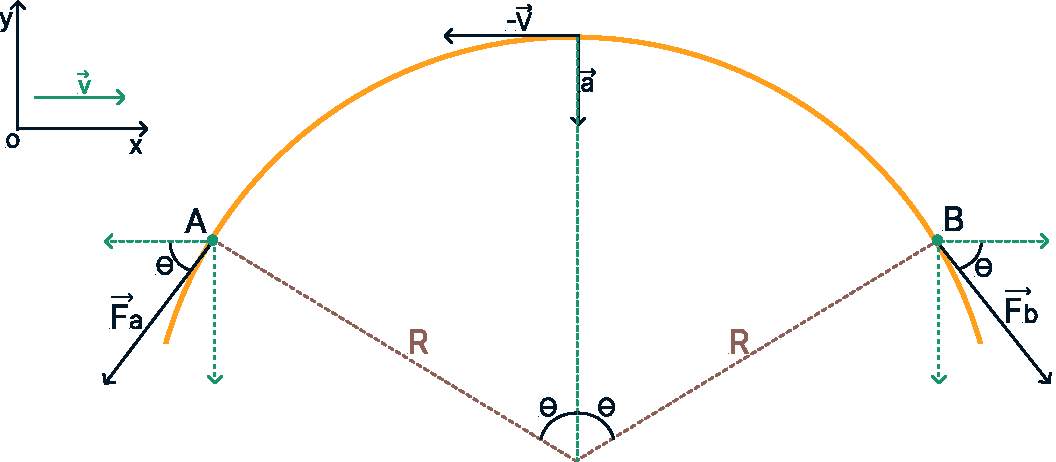
\includegraphics[width=.7\paperwidth]{images/graph_forces.pdf}

    Dans le morceau de corde apparaît un MCU avec une norme de vitesse $V$.
    \\
    \newline
    Selon la deuxième loi de Newton:
    \begin{center}
        \vspace{-\baselineskip}
        \begin{minipage}[t][1.75cm][t]{0.4\linewidth}
            \begin{empheq}[box={\mymath}]{align*}
                F_a\sin(\theta) + F_b\sin(\theta) &= ma
            \end{align*}
        \end{minipage}%
        \begin{minipage}[t][1.75cm][t]{0.4\linewidth}
            \begin{empheq}[box={\mymath}]{align*}
                2F_T\sin(\theta) &= m\frac{v^2}{R}
            \end{align*}
        \end{minipage}
    \end{center}
    Où $R$ est le rayon du cercle dont l'arc $AB$ fait partie.
    \newline

    Noter que $m$ peut également être écrit comme:
    
    \begin{empheq}[box={\mymath}]{align*}
        m &= \mu l
    \end{align*}

    Où

    \begin{empheq}[box={\mymath}]{align*}
        l &= R2\theta
    \end{align*}
    \newline
    On considère que $\theta$ aura des valeurs faibles, donc $\sin(\theta) \approx \theta$.
    En conséquence :
    \begin{empheq}[box={\mymath}]{align*}
        2 \cdot F_T \cdot \theta &= \mu \cdot R \cdot 2 \cdot \theta \cdot \frac{v^2}{R}
    \end{align*}
    Devient:
    
    \begin{center}
        \vspace{-\baselineskip}
        \begin{minipage}{0.4\linewidth}
            \begin{empheq}[box={\mymath}]{align*}
                F_T &= \mu v^2
            \end{align*}
        \end{minipage}%
        \begin{minipage}{0.1\linewidth}
            Ou
        \end{minipage}%
        \begin{minipage}{0.3\linewidth}
            \begin{empheq}[box={\mymath}]{align*}
                v &= \frac{F_T}{\mu}
            \end{align*}
        \end{minipage}
    \end{center}

    \subsubsection{Ondes progressives}
    D'un point de vue mathématique, les ondes peuvent être décrites par une fonction $y$ qui accepte deux paramètres $(x,t)$.

    \begin{empheq}[box={\mymath}]{align*}
        y(x,t) &= f(x \pm vt)
    \end{align*}
    
    \begin{itemize}
        \item Avec \bf{-} onde progressive vers $x$ positif
        \item Avec \bf{+} onde progressive vers $x$ négatif
    \end{itemize}

    \subsubsection{Ondes sinusoïdales progressives}

    \begin{empheq}[box={\mymath}]{align*}
        y(x,t) &= A\sin(kx \pm wt + \varphi)
    \end{align*}


    \begin{center}
        \vspace{-\baselineskip}
        \begin{minipage}{0.4\linewidth}
            \begin{empheq}[box={\mymath}]{align*}
                \frac{dx}{dy}y
            \end{align*}
        \end{minipage}%
        \begin{minipage}{0.1\linewidth}
            \Rightarrow
        \end{minipage}%
        \begin{minipage}{0.3\linewidth}
            \begin{empheq}[box={\mymath}]{align*}
                v &= \frac{\lambda}{T} = \lambda f
            \end{align*}
        \end{minipage}
    \end{center}

    Où

    \begin{itemize}
        \item $\lambda$ - Longueur d'onde
        \item $T$ - Période d'oscillation
        \item $f$ - Fréquence d'oscillation
    \end{itemize}

    \subsubsection{Ondes stationnaires dans une corde attachée aux extrémités}

    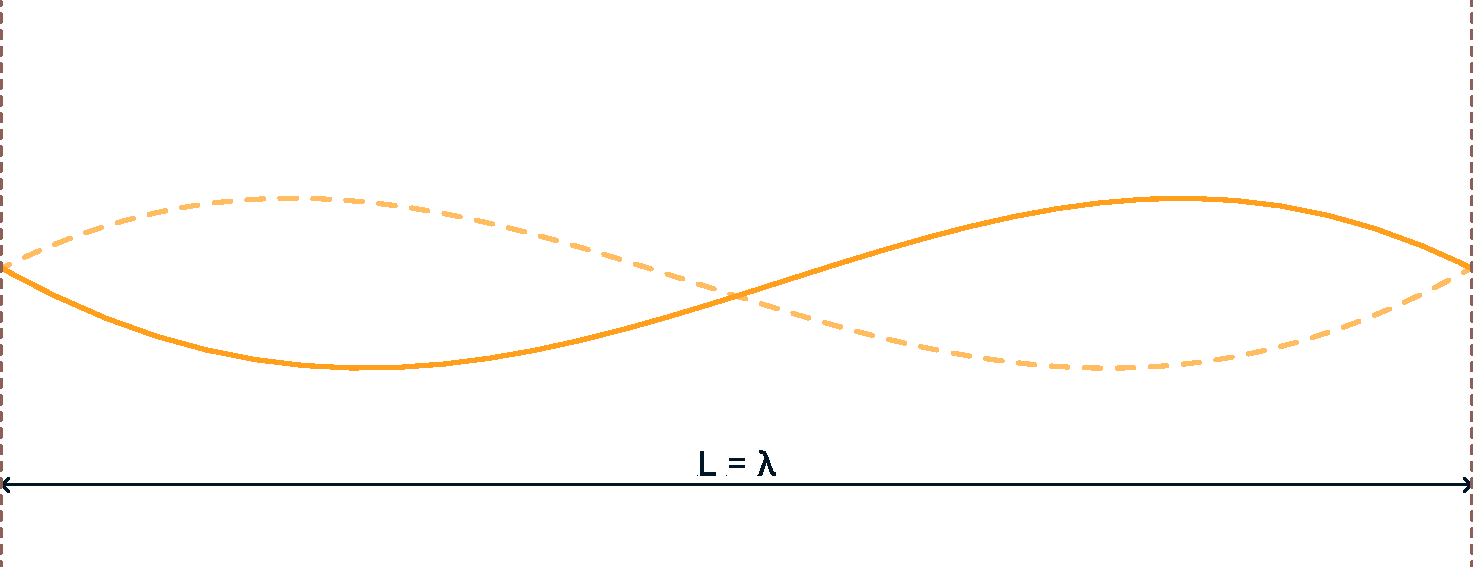
\includegraphics[width=.35\paperwidth]{images/graph_l_lambda.pdf}
    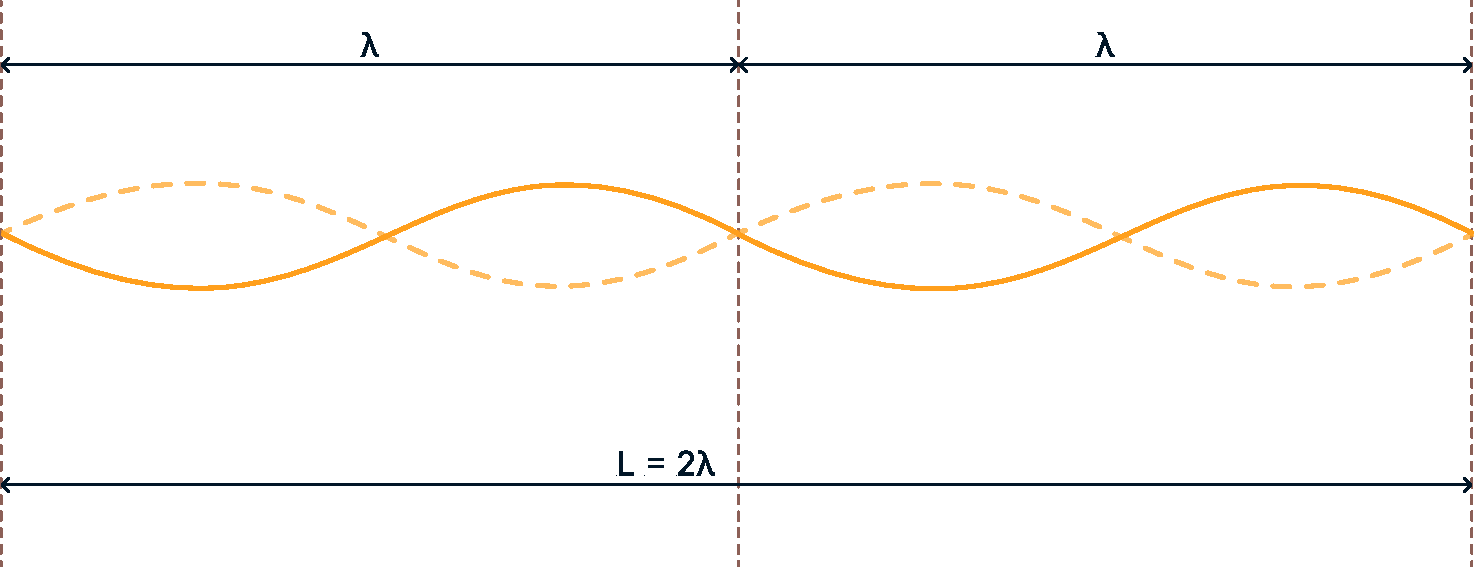
\includegraphics[width=.35\paperwidth]{images/graph_l_2lambda.pdf}

    \begin{center}
        \vspace{-\baselineskip}
        \begin{minipage}{0.4\linewidth}
            \begin{empheq}[box={\mymath}]{align*}
                \lambda_1 &= 2L
            \end{align*}
        \end{minipage}%
        \begin{minipage}{0.1\linewidth}
            \Rightarrow
        \end{minipage}%
        \begin{minipage}{0.3\linewidth}
            \begin{empheq}[box={\mymath}]{align*}
                f_1 &= \frac{v}{2L}
            \end{align*}
        \end{minipage}
    \end{center}

    \begin{center}
        \vspace{-\baselineskip}
        \begin{minipage}{0.4\linewidth}
            \begin{empheq}[box={\mymath}]{align*}
                \lambda_2 &= L
            \end{align*}
        \end{minipage}%
        \begin{minipage}{0.1\linewidth}
            \Rightarrow
        \end{minipage}%
        \begin{minipage}{0.3\linewidth}
            \begin{empheq}[box={\mymath}]{align*}
                f_2 &= \frac{v}{L}
            \end{align*}
        \end{minipage}
    \end{center}
    \begin{center}
        \vspace{-\baselineskip}
        \begin{minipage}{0.4\linewidth}
            \begin{empheq}[box={\mymath}]{align*}
                \lambda_3 &= \frac{2L}{3}
            \end{align*}
        \end{minipage}%
        \begin{minipage}{0.1\linewidth}
            \Rightarrow
        \end{minipage}%
        \begin{minipage}{0.3\linewidth}
            \begin{empheq}[box={\mymath}]{align*}
                f_3 &= \frac{3v}{2L}
            \end{align*}
        \end{minipage}
    \end{center}

    \begin{center}
        ...
    \end{center}

    \begin{center}
        \vspace{-\baselineskip}
        \begin{minipage}{0.4\linewidth}
            \begin{empheq}[box={\mymath}]{align*}
                \lambda_n &= \frac{2L}{n}
            \end{align*}
        \end{minipage}%
        \begin{minipage}{0.1\linewidth}
            \Rightarrow
        \end{minipage}%
        \begin{minipage}{0.3\linewidth}
            \begin{empheq}[box={\mymath}]{align*}
                f_n &= \frac{nv}{2L}
            \end{align*}
        \end{minipage}
    \end{center}
    



    \subsection{Principe de l'expérience}
    L'expérience consiste en ces deux parties :
    \begin{enumerate}
        \item Avant de procéder à l'expérience proprement dite, on calcule la masse linéique de la corde à l'aide de différentes mesures liées au poids et à la corde, qu'on utilise ensuite, avec la force $F$, pour calculer la vitesse $v_{calc}$.
        \item On mesure les paires de ($n$, $f_n$) pour les douze premières harmoniques, puis on les utilise pour construire une régression linéaire, à partir de la pente de laquelle on extrait la vitesse $v_{exp}$.
    \end{enumerate}

    \subsection{Schéma et montage de l’expérience}
    Pour réaliser l'expérience, on a besoin d'un vibreur qui fait vibrer une corde à différentes fréquences. une extrémité de la corde est attachée au vibreur et l'autre passe dans une poulie. Un poids est accroché à la corde afin de la maintenir en tension.
    \\
    Dans notre cas, on a utilisé :
    \begin{itemize}
        \item Une corde
        \item Un vibreur à fréquence variable
        \item Une poulie
        \item Des barres pour fixer le vibreur et la poulie
    \end{itemize}  
    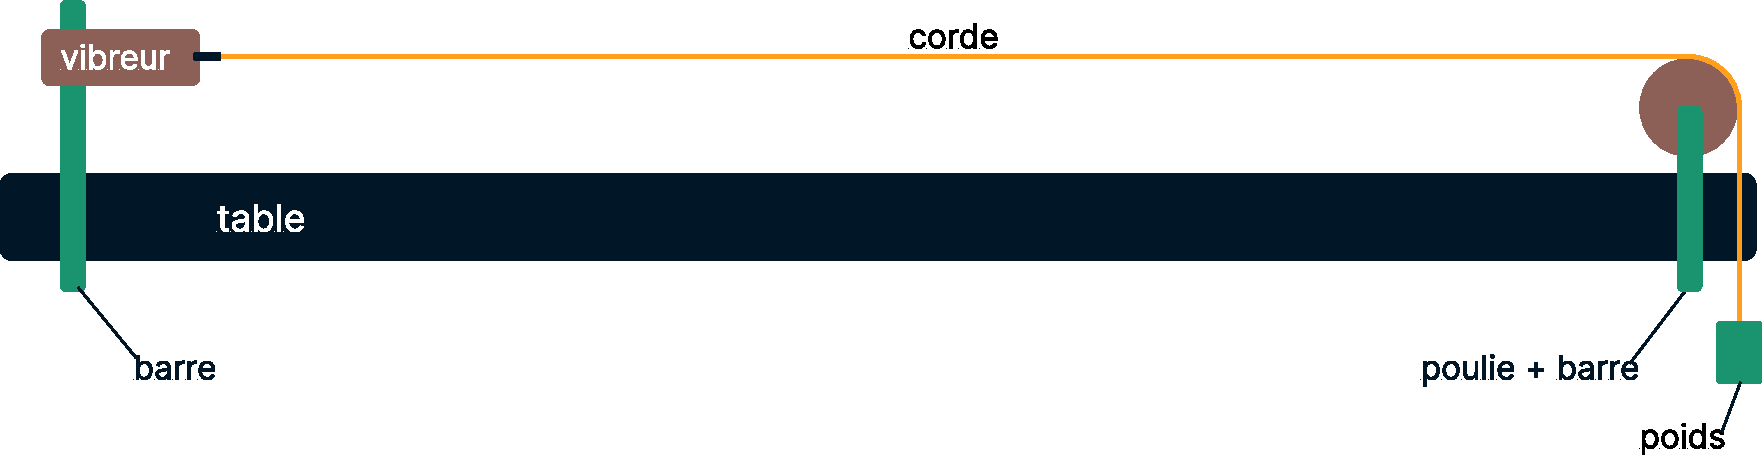
\includegraphics[width=0.35\paperwidth]{images/schema_static.pdf}
    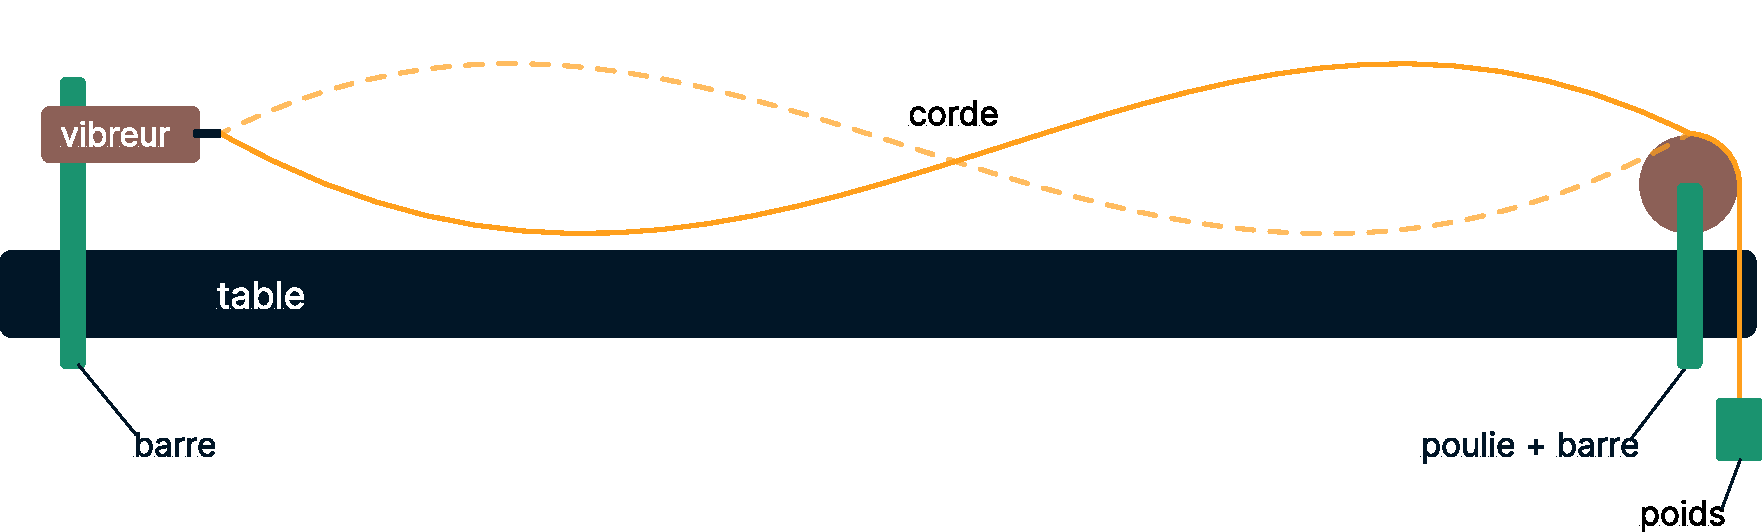
\includegraphics[width=0.35\paperwidth]{images/schema_dynamic.pdf}
    \subsection{Déroulement de l'expérience}
    \subsubsection{Les mesures préalables}
    \begin{itemize}
        \item On prend une balance et on mesure la masse totale de la corde.
        \item On établit une longueur étalon, qui servira à calculer le coefficient d'allongement de la corde.
        \item Avec cette longueur initiale, on calcule la longueur de la corde après avoir attaché le même poids que on utilise plus tard pour mettre en place l'expérience.
    \end{itemize}
    \subsubsection{Le calcul des harmoniques}
    \begin{itemize}
        \item On met l'agitateur sur une tige fixée à la table de travail.
        \item En prenant une distance considérable, on met une poulie de la même manière.
        \item On attache et on place la corde entre l'agitateur et la poulie, et on la tend à l'aide d'un poids à l'extrémité libre.
        \item On mesure la distance résultante entre l'extrémité de l'agitateur et la poulie.
        \item On connecte l'agitateur à un générateur de courant alternatif réglable.
        \item En ajustant la fréquence et la tension (amplitude) du générateur, on génère les douze premières harmoniques du notre système.
    \end{itemize}
    \newpage
    \section{Mesures}
    \subsection{Mesures constantes :}
    \begin{itemize}
        \item $L=(1.79 \pm 0.05)$ m - longueur entre l'agitateur et la poulie
        \item $m=(199.6 \pm 0.1)$ g - poids pour la fixation de la corde
        \item $m_c=(10.3 \pm 0.1)$ g - masse de la corde
        \item $l'=(0.39 \pm 0.03)$ m - longueur de la corde avant l'étirement
        \item $l''=(0.43 \pm 0.03)$ m - longueur de la corde après l'étirement
    \end{itemize}
    \subsection{Tableau des mesures :}

    \begin{minipage}{0.4\textwidth}
        \centering
        \begin{tabular}{c|c|c}
            \toprule
            $n$ & $f_n$ (Hz)  & $\Delta f_n$ (Hz) \\
            \midrule
            1  & 6.37  & 0.02 \\
            2  & 13.18 & 0.02 \\
            3  & 19.68 & 0.02 \\
            4  & 26.21 & 0.02 \\
            5  & 32.51 & 0.02 \\
            6  & 39.51 & 0.02 \\
            7  & 45.71 & 0.02 \\
            8  & 52.81 & 0.02 \\
            9  & 59.21 & 0.02 \\
            10 & 65.71 & 0.02 \\
            11 & 72.51 & 0.02 \\
            12 & 78.71 & 0.02 \\
            \bottomrule
        \end{tabular}
        \captionof{table}{Les douze premières harmoniques}
    \end{minipage}%
    \hfill
    \begin{minipage}{0.6\textwidth}
        Légende :
        \begin{itemize}
            \item $n$ - nombre de l'harmonique
            \item $f_n$ - fréquence de l'harmonique $n$ (en Hz)
            \item $\Delta f_n$ - incertitude de la fréquence (en Hz)
        \end{itemize}
    \end{minipage}

    \newpage
    \section{Analyse des mesures et résultats}
    \subsection{Vitesse avec la masse linéique}
    Pour calculer la vitesse à l'aide de la force $F$ et la masse linéique $\mu$, on utilise la formule de la partie théorique :
    \begin{empheq}[box={\mymath}]{equation*}
        v_{calc} = \sqrt{\frac{F}{\mu}}
    \end{equation*}
    On obtient, donc :
    \begin{empheq}[box={\mymath}]{equation*}
        v_{calc} = (20 \pm 6) \textrm{ ms}^{-1}
    \end{equation*}
    \subsection{Vitesse avec les harmoniques}
    Pour construire la régression linéaire, on partira de la formule suivante déduite dans la partie théorique :
    \begin{empheq}[box={\mymath}]{equation*}
        f_n = \frac{v_{exp}}{2L} \cdot n
    \end{equation*}
    On constate que la valeur $f_n$ est une fonction de $n$, et on voit aussi que $\frac{v_{exp}}{2L}$ est la pente de la fonction, qu'on note par $a$ pour les calculs qui suivre. \\ 
    On obtient, donc :
    
    \pgfplotstableread[col sep=comma]{data/exp_data.csv}\expIdata
    \begin{tikzpicture}[scale=1]
        % Scatter plot
        \begin{axis}[
            xlabel={$n$},
            ylabel={$f_n$ (Hz)},
            legend pos=north east,
            legend style={at={(0.30,0.75)}, anchor=south},
            grid=both,
            width=1\textwidth,
            height=0.3\textheight,
            x tick label style={
                /pgf/number format/.cd,
                precision=0,
                fixed,
                fixed zerofill,
            },
            y tick label style={
                /pgf/number format/.cd,
                precision=2,
                fixed,
                fixed zerofill,
            },
            xmin=0,
            xmax=13,
            ymin=4,
            ymax=81,
        ]
            \addplot+[only marks, mark=x, error bars/.cd, x dir=both, x explicit, y dir=both, y explicit] table[x=n, x error=err_g, y=fn, y error=err_fn] {\expIdata};

            % Linear regression line
            \addplot [red, thick] table[
                y={create col/linear regression={y=fn}}
            ] {\expIdata};
            \xdef\slope{\pgfplotstableregressiona}
            \xdef\intercept{\pgfplotstableregressionb}

            % Add the equation of the line
            \addlegendentry{Données}
            \addlegendentry{Régr. Lin.: $y = \pgfmathprintnumber{\slope}x + \pgfmathprintnumber{\intercept}$}
        \end{axis}
    \end{tikzpicture}
    Après avoir extrait la vitesse et l'incertitude de la valeur 
de la pente, on a :
    \begin{empheq}[box={\mymath}]{equation*}
        v_{exp} = (23.6 \pm 0.8) \textrm{ ms}^{-1}
    \end{equation*}

    \newpage
    \subsection{Choix et calcul d'incertitudes}
    \subsubsection{Choix des incertitude :}
    \begin{itemize}
        \item Pour la longueur de la corde : lorsque la longueur est proche de 2 mètres, notre précision diminue, on a donc choisi une incertitude plus grande de $\Delta L = 0.05$ m.
        \item Pour les deux longueurs $l'$ et $l''$ : compte tenu du fait que les mesures ont été effectuées sur de petites distances, on a choisi une incertitude $\Delta l = 0.03$ m.
        \item Pour les masses : on utilise l'incertitude indiquée par la balance $\Delta m = 0.01$ g.
        \item Pour l'incertitude de la fréquence : dans ce cas, l'incertitude peut provenir de plusieurs facteurs :
        \begin{itemize}
            \item On ne sait pas si l'agitateur répond exactement à la fréquence indiquée par le générateur.
            \item On ne sait pas si cette fréquence est exactement la fréquence correspondant à l'harmonique $n$.
        \end{itemize}
        Ainsi, par expérience, on a observé qu'il n'y a pas de changement visible dans la forme de l'harmonique si on change la fréquence de $\pm 0.02$ Hz.
    \end{itemize}
    \subsubsection{Calcul d'incertitudes}
    On sait que $v_{calc}$ est représenté par la formule :
    \begin{empheq}[box={\mymath}]{equation*}
        v_{calc} = \sqrt{\frac{F}{\mu}}
    \end{equation*}
    On peut donc calculer l'incertitude à l'aide du calcul suivant :
    \begin{empheq}[box={\mymath}]{equation*}
        \frac{\Delta v_{calc}}{|v_{calc}|} = \frac{1}{2} \cdot \frac{\Delta F / \mu}{|F / \mu|}
    \end{equation*}
    On sait que :
    \begin{align*}
        \begin{cases}
            F &= mg \\
            \mu &= \frac{m_c}{L} \cdot \frac{l'}{l''}
        \end{cases}
        & \Rightarrow
        \begin{cases}
            \Delta F &= 1 \, \text{mN} \\
            \Delta \mu &= 2 \, \text{gm}^{-1}
        \end{cases}
    \end{align*}
    Donc:
    \begin{empheq}[box={\mymath}]{equation*}
        \Delta v_{calc} = 6 \textrm{ ms}^{-1}
    \end{equation*}
    Pour calculer l'incertitude de $v_{exp}$, on va utiliser quelques notions de statistiques simples :
    \begin{itemize}
        \item On connait l'erreur standard de la pente : $err_{st} \approx 0.016$
        \item On admet que on a une confiance de $95\%$ dans nos résultats, donc on a une valeur critique de $val_{crt} \approx 1.96$
    \end{itemize}
    On en déduit la formule suivante :
    \begin{empheq}[box={\mymath}]{equation*}
        \Delta a = err_{st} \cdot val_{crt} = 0.04
    \end{equation*}
    En utilisant la pente, on a donc le calcul suivant :
    \begin{align*}
        \frac{\Delta v_{\text{exp}}}{v_{\text{exp}}} = \frac{\Delta a}{a}& + \frac{\Delta (2L)}{2L} \\
        \Downarrow&
    \end{align*} %
    \begin{empheq}[box={\mymath}]{equation*}
        \Delta v_{\text{exp}} = 0.8 \, \text{ms}^{-1}
    \end{empheq}
    \subsection{Discussion des résultats :}
    On a obtenu deux valeurs pour la vitesse:
    \begin{align*}
        v_{exp} = (23.6 \pm 0.8) \textrm{ ms}^{-1}
        & \textrm{ et }
        v_{calc} = (20 \pm 6) \textrm{ ms}^{-1}
    \end{align*}
    Ces résultats nous permettent de tirer les conclusions suivantes sur la manière de les atteindre :
    \begin{itemize}
        \item En utilisant la masse linéique $\mu$ et la force de la pesanteur $F$ :
        \begin{itemize}
            \item Cette façon d'obtenir la vitesse est très facile à mettre en pratique, car on n'a pas besoin d'une installation compliquée pour obtenir les mesures nécessaires.
            \item L'inconvenient de cette méthode est que le résultat est très imprécis (on a obtenu une incertitude de 6 ms$^{-1}$, ce qui représente presque la moitié de la valeur obtenue pour la vitesse elle-même, et  pour des calculs plus prècis cela peut coûter cher).
            \item L'incertitude élevée provient du fait que la formule elle-même dépend de nombreux produits, divisions et calculs avec des puissances :
            \begin{equation*}
                v_{calc} = \sqrt{\frac{F}{\mu}} = \sqrt{\frac{mgL}{m_c} \cdot \frac{l''}{l'}}
            \end{equation*}
        \end{itemize}
        \item En faisant une régression linéaire avec les $n$ premières harmoniques :
        \begin{itemize}
            \item Cette méthode d'obtenir la vitesse est beaucoup plus précise que la précédente (une incertitude de 0.8 ms$^{-1}$ au lieu de 6 ms$^{-1}$), parce que on n'a que l'incertitude de la fréquence et de la longueur de l'installation qui affecte le résultat final.
            \item L'inconvenient de cette méthode est que l'expérience nécessite beaucoup plus de préparation que la précédente, et que de nombreux facteurs peuvent conduire à des mesures qui s'écartent des valeurs idéales (par exemple, on ne sait pas si l'agitateur répond à la même fréquence que celle affichée sur le générateur).
            \item On a toujours une incertitude assez élevée, car il este très difficile de prédire si la fréquence que on a récoltée est vraiment la fréquence théorique de l'harmonique que on génere.
        \end{itemize}
    \end{itemize}
    En général, les deux méthodes sont deux bons outils pour calculer la vitesse, le seul facteur qui influence le choix de l'une des deux étant le niveau de précision dont on a besion dans les calculs que on fait ensuite avec cette vitesse.
    \section{Synthèse et conclusion}
    Dans ce laboratoire, on a cherché à comprendre le comportement des ondes stationnaires et à appliquer les formules données par la théorie. \\
    Afin de réaliser cet objectif, on a calculé la vitesse de propagation d'une onde de deux manières différentes :
    \begin{itemize}
        \item En utilisant la masse linéique de la corde $\mu$ et la force de pesanteur $F$.
        \item En collectant des paires ($n$, $f_n$) pour les douze premières harmoniques de l'onde, puis en les utilisant pour construire une régression linéaire.
    \end{itemize}
    Le résultat de cette expérience est que on a démontré que on dispose de deux outils pratiques pour calculer cette vitesse, qui présentent différents niveaux de difficulté d'application et de précision des résultats. \\
    En utilisant et en comparant les résultats des ces deux méthodes de calcul, on a également confirmé que les formules déduites par le raisonnement théorique correspondent à des résultats réels et tangibles.
\end{document}

